\documentclass{article}
\usepackage{amsmath}
\usepackage{float}
\usepackage{amssymb}
\usepackage{graphicx}
\usepackage[margin=1in]{geometry}
\usepackage{multicol,caption,listings}
\usepackage{cite}

\bibliographystyle{plain}

\begin{document}

\title{Polymer Chain Monte Carlo}
\author{A. Lovell}
\maketitle

\noindent \textbf{Abstract}  Write the abstract here - give a brief overview about what you have done and what you're planning on showing.

\begin{multicols}{2}

\section{Introduction}

Polymer are chains atoms or molecules of the same type that interact directly between sequential atoms through a spring force and through other pairs via some other long- or short-range potential (given, for example, by hydrogen bonds, van der Waals interactions, or the Lennard-Jones interaction).  The typical number of atoms in a polymer is between $10^3$ and $10^5$.  \\

One would often think that a molecular dynamics calculation would be used to simulate a polymer chain.  In this case, the movement of the chain would be calculated at each time step, the forces between each molecule calculated, and then used to update the chain's next position.  However, because of the different types of motion involved in the problem - ranging from fast motion of the individual units to slow motion of the chain as a whole - this process can be inefficient, or even impossible, for long chains.  \cite{PhilNotes} Instead, Monte Carlo simulations are used to discover properties of the polymer.  \\

This report is broken up into the following sections.  In Section \ref{theory}, we will discuss the theory behind the problem, including the interaction between atoms and the algorithm that was used to run the Monte Carlo simulation.  Section \ref{IC} gives a brief discussion of the initial conditions of the simulation and the different grids that were explored.  The results of the simulation are discussed in Section \ref{discuss}.  Finally, in Section \ref{concl}, we provide a summary of our work along with progress that could be make to this project in the future. \\

\section{Theory}
\label{theory}

In the following section, we will describe some of the concepts that will be needed to simulate a polymer chain.

\subsection{Interaction}

Polymer chains can be modeled in several ways.  One of the most common ways is describing the interaction between sequential pairs of atoms as a stiff spring and putting in a Lennard-Jones potential between every other pair of atoms.  \textbf{Reference this.}  However, in this project we will take a somewhat simplified approach.  Instead of stiff springs, we will fix the length between each successive pair of atoms, while keeping the interaction between all other pairs a Lennard-Jones interaction.  There are, of course, more complicated that could be implemented to fold the polymer into more complex shapes (such as proteins or even origami ducks), but those will not be explored here.\\

The Lennard-Jones interaction is 

\begin{equation}
\label{VLJ}
V_{LJ}(r) = 4\epsilon \left [ \left ( \frac{\sigma}{r} \right ) ^{12} - \left ( \frac{\sigma}{r}) \right ) ^6 \right ]
\end{equation}

\noindent where $\epsilon$ is the depth of the interaction, $\sigma$ describes the particle size, and $r$ is the distance between the interacting pairs.  When the two atoms are far enough apart, they can be viewed as non-interacting.  For this reason, we can introduced a cut-off radius, $r_c$, beyond which the potential between two particles is taken to be zero.  Thus, we use the interaction 

\begin{equation}
V_{LJ} (r) = \begin{cases}
4 \epsilon \left [ \left (\frac{\sigma}{r} \right )^{12} - \left (\frac{\sigma}{r} \right )^{6} \right ] & r \le r_c \\
0 & r > r_c
\end{cases}
\label{cutoff}
\end{equation}

This form takes into account the short-range repulsive force between the two atoms due to Coulomb repulsion and the longer-range attractive forces from dipole-dipole and dipole-induced dipole forces.  An example of the Lennard-Jones potential can be found in Figure \ref{VLJfig}.

\begin{figure}[H]
\begin{center}
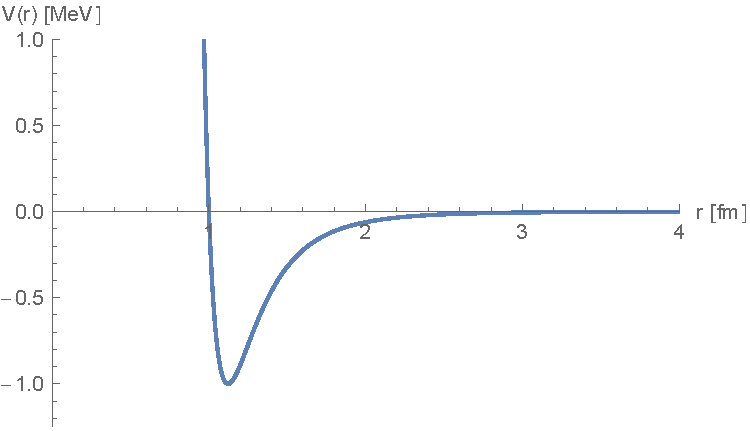
\includegraphics[width=\linewidth]{Figures/VLJ.pdf}
\caption{The shape of the Lennard-Jones potential.  Here, $\sigma=1$ fm (the distance where the potential crosses the r-axis) and $\epsilon =1$ MeV (the maximum depth of the interaction).}
\label{VLJfig}
\end{center}
\end{figure}

\subsection{Algorithm}

The algorithm that we use to pick the next point for this Monte Carlo simulation is the Rosenbluth algorithm proposed in 1956 by Marshall and Arianna Rosenbluth.  As compared to simple sampling - which generates all configurations with equal probability - the Rosenbluth algorithm generates configurations with different probabilities.  These probabilities cause the chain to be self-avoiding and make it so that it terminates when it is trapped in a dead end.  \cite{SSRosenbluth} \\

On a square (or cubic) lattice, this means that each nearest neighbor is tested as to whether or not it is already occupied, and the the probability that it moves to that cite is based on the energy of the potential new configuration using the statistical factor

\begin{equation}
\label{prob}
P_i = \frac{1}{Z} e^{-V_i/T}
\end{equation}

\noindent where

\begin{equation}
\label{part}
Z = \sum \limits _{i=1}^{N_a} e^{-V_i/T}
\end{equation}

\noindent Here, $V_i$ is the potential energy between the $i^{th}$ potential configuration and the rest of the chain, $N_a$ is the number of unoccupied nearest neighbors, and T is the temperature of the system.  These probabilities are mapped onto the range $[0,1]$, and a random number is picked within that same range.  If this random number falls within the range $P_i$, then the next atom is added at the position from which $V_i$ was calculated.  \\

However, we can also grow our polymer off of a grid.  In this case we have to sample from a circle in two-dimensions or a sphere in three-dimensions.  Do do this we sample from $\mathrm{cos}\theta \in [-1,1]$ and $\phi \in [0,2\pi]$ (taking $\theta = \pi/2$ for the two-dimensional case, to fix the third dimension).  This samples over the circumference of a unit circle in two-dimensions and the surface of a sphere in three-dimensions.  Some number, $N_a$, of the points are randomly chosen, and new positions are calculated based on 

\begin{equation}
\begin{split}
x^{j}_i & = x^{j-1} + \mathrm{sin}\theta _i \mathrm{cos}\phi _i \\
y^{j}_i & = y^{j-1} + \mathrm{sin} \theta _i \mathrm{sin} \phi _i \\
z^{j}_i & = z^{j-1} + \mathrm{cos} \theta _i
\end{split}
\end{equation}

\noindent The probabilities for each $\textbf{r}_i$ to be chosen is the same as described above with equations (\ref{prob}) and (\ref{part}).

\subsection{Configuration}

The main quantity that we want to calculate is the relationship between the size of the system and the number of atoms in the polymer, which should be related to the dimensionality of the simulation (e.g. two-, three-, or more dimensional space).  To do this, we relate the gyromagnetic radius, $R_g$, to the number of atoms in the chain, $N$, where 

\begin{equation}
R_g^2 = \frac{1}{N} \sum \limits _{i=1}^{N} \langle (r_i - R_{cm})^2 \rangle
\end{equation} 

\noindent and 

\begin{equation}
\label{RNcomparison}
R \sim N^{\nu}
\end{equation}

The temperature, $T_{\Theta}$, defines the transition between a chain-like polymer ($T<T_{\Theta}$) and a dense, ball-like polymer ($T>T_{\Theta}$).  Below $T_{\Theta}$, $\nu = 1/ 2$, at $T_{\Theta}$, $\nu = 1/3$, and above $T_{\Theta}$, $\nu$ scales with the dimensionality of the simulation - namely, $\nu = 3/(d+2)$, where $d$ is the dimensionality of the simulation.  \\

\textbf{CITE THIS!!!!!!} \\

This is the main observable we will be calculating for this Monte Carlo simulation.  From this, we can also define the $\Theta $-temperature, $T_{\Theta}$.

\section{Initial Conditions}
\label{IC}

The first two atoms of the chain were positioned at (0,0,0) and (1,0,0).  Essentially, these positions are arbitrary (only constrained to be 1 unit length apart), but it gives a good starting point for both the polymer on a grid and in free space.   \\

In this calculation, we also chose $\epsilon =1$ and $\sigma=1$ in (\ref{VLJ}).  In order to compare to data from the lab, we would just need to change our potentials to include realistic numbers for these two values.  Along with this, we also are using units where $k_B=1$.  This gives us temperature in eV, with $1 K \approx 11600$ eV.  Thus, even seemingly small temperatures become large quickly.

\section{Discussion}
\label{discuss}

In this section, we present the main result of our calculation.  We were able to vary the temperature of the polymer, from 1.0 eV to 5.0 eV, as well as the number of atoms, $N=5000, 10000, 15000$, to calculate the radius of gyration and see how well our simulation compares to (\ref{RNcomparison}).  These results are summarized in Table 1.  \\

\begin{table*}
\begin{center}
\begin{tabular}{| c | c | c | c | c | c | c |}
\hline & $T=1.0$ eV &  & $T=2.0$ eV &  & $T=5.0$ eV & \\ \hline
 & \textbf{$R_g$} & \textbf{$\sigma _{R_g}$} & \textbf{$R_g$} & \textbf{$\sigma _{R_g}$} & \textbf{$R_g$} & \textbf{$\sigma _{R_g}$} \\ \hline
$N=5000$ & 2.5119 & 0.343484 & 3.109664 & 0.312228 & 3.308621 & 0.330394 \\ \hline
$N=10000$ & 2.783211 & 0.295998 & 3.656107 & 0.335429 & 3.642807 & 0.321192 \\ \hline
$N=15000$ & 2.994968 & 0.376915 & 3.722428 & 0.343053 & 3.872835 & 0.318437 \\ \hline
\end{tabular}
\label{results}
\caption{Results for a three-dimension polymer chain in free space (not on a grid) for three different temperatures at three different polymer lengths.  Both the mean value and the standard deviation for each set of points is given.}
\end{center}
\end{table*}

In Figure \ref{}, we show the results of the simulation plotted along with the best fit line for each set of data.  These fits are given in Table 2.  \\

\begin{table*}
\begin{center}
\begin{tabular}{| c | c | c | c |}
\hline \textbf{T (eV)} & \textbf{m (fm)} & \textbf{b (fm)} & \textbf{$\chi ^2$} \\ \hline
1.0 & 0.4345 & -1.1968 & \\ \hline
2.0 & 0.5826 & -1.8139 & \\ \hline
5.0 & 0.5102 & -1.042 & \\ \hline
\end{tabular}
\caption{Slopes ($m$) and y-intercepts ($b$) for the best fit lines for the simulation data in Table 1.  Best fit lines are given as $log(R_g) = m*log(N) + b$.  Here $log$ indicates the natural log.  In this case, the slope $m$ gives the value for $\nu$ from (\ref{RNcomparison}).}
\end{center}
\end{table*}

From these fits, we find that $\nu = 0.4345$ for $T=1.0$ eV, $\nu = 0.5826$ for $T = 2.0$ eV, and $\nu = 0.5102$ for $T = 5.0$ eV.  The first two cases match up well with a temperature just below $T_{\Theta}$ for $T=1.0$ eV and for a temperature above $T_{\Theta}$ that follows the pattern $\nu = 3/(d+2)$ for $T = 2.0$ eV.  (Recall, for this simulation $d=3$ so $\nu = 0.6$.)  However, we see that for $T = 5.0$ eV, $\nu \approx 0.5$ which would seem to indicate that this is the $\Theta$-temperature. This cannot be the case.  To explain this, we note that $5.0$ eV $\approx 58000$ K, which is an order of magnitude hotter than the coolest part of the sun.  \cite{sun}  We assume that at these temperatures, our simple model is no longer valid, and we get nonsensical results from our calculations.  \\

Still, in the region where our simulation is valid, we have calculated reasonable results for our three-dimensional simulation of a polymer chain.  

\section{Conclusion}
\label{concl}

Talk briefly about what we calculated.  \textbf{Varying size, varying dimension, varying temperatures - find the critical temperature Theta.}\\

There is always future work that could be done regarding this project.  While we calculated a polymer chain in three-dimensions, it would also be interesting to calculate higher dimensional chains and examine the scaling of the size of the chain with the number of atoms added to the chain.  The same results as \textbf{(put reference to either equations or figures)} should hold, but it would be an interesting project nonetheless to generalize the code.  It would also be interesting to examine the difference between this free self-avoiding walk calculated here and a self-avoiding walk confined to a grid.  In this way, we could see how the size of the polymer is related to the number of atoms and the dimensionality of the problem.  \\

There are also several thermodynamical quantities that could be calculated from this system, including specific heat, thermal energy, and \textbf{many more}.  Although we used a fixed bond length between each successive atom and a Lennard Jones interaction between all pairs of atoms, there are many other interactions that could describe a more realistic polymer.  This includes using a stiff spring to model the interaction between successive atoms.  We also could have changed the strength of the interaction between various pairs to see what kinds of shapes we could form with our polymer chain.  Still, we successfully modeled a polymer chain of \textbf{N} atoms in \textbf{two-} and three-dimensions.  \\

\textbf{Mention PERM, more accurate way of calculating these things.}

\appendix

\section{Error Analysis}

Just as experimentally measured data points should quote errors - whether due to systematics, timing, or unknown quantities - theoretical simulations and calculations should also quote error bars.  To do this, we run our simulation several times to find a mean value and a standard deviation.  The mean is calculated by

\begin{equation}
\bar x = \frac{1}{N} \sum \limits _{i=1}^N x_i
\end{equation}

\noindent where $\bar x$ is the mean value, $x_i$ are the values of a given quantity from each calculation (for instance the length of the chain), and $N$ is the number of simulations run.\\

To find the error on each data point, we average the standard deviation for each run.

\begin{equation}
\label{stddev}
\sigma _x^2 = \frac{1}{N} \sum \limits _{i=1} ^N (x_i - \bar x)^2
\end{equation}

\noindent Here, $\sigma _x$ is the error for the variable $x$ from each calculation.  We can see that the errors decrease as $1/\sqrt{N}$.  \\

Because we are calculating a fit to data, we should also report a $\chi ^2$ value for that fit, to assess its "goodness" - or the quality of the fit when compared to data.  \cite{Nunes}  In this case, we would calculate the $\chi^2$ of each of the linear fits that are made to the simulation "data".

\begin{equation}
\chi ^2 = \sum \limits _{i=1} ^N \frac{(x^{sim} - x^{fit})^2}{\sigma _x ^2}
\end{equation}

\noindent In this case, $x^{sim}$ is the parameter value from the simulation, $x^{fit}$ is the parameter value from the fit through the simulation data, and $\sigma _x ^2$ is the square of the standard deviation (the variance) from (\ref{stddev}). \\

Although this does not give us an error on the fits that are being made, it does give some indication as to the quality of the fit.

\end{multicols}

\bibliography{chainbib}

\end{document}